\section{Analog-Digital-Wandler (ADC)}

\begin{minipage}[c]{0.48\columnwidth}
    \begin{tabular}{ll}
        $n$         & Anzahl Bits                       \\
        $D$         & Digitaler Wert \quad $D < 2^n$    \\
        $q$         & Quantisierungsschritt             \\
        $B_0$       & Bitwert 0 (LSB)                   \\
        $B_{n-1}$   & Bitwert $n-1$ (MSB)
    \end{tabular}
\end{minipage}
\hfill
\begin{minipage}[c]{0.48\columnwidth}
    $$ \boxed{ q = \frac{V_{\rm refp} - V_{\rm refn}}{2^n} } $$
    $$ \boxed{ D = \frac{V_{\rm in} - V_{\rm refn}}{V_{\rm refp} - V_{\rm refn}} \, 2^n } $$
\end{minipage}


\subsection{Einführung}

\begin{itemize}
    \item Ein AD-Wandler ordnet einer analogen Spannung einen digitalen Wert zu
    \item Der einfachste AD-Wandler ist ein Komparator (1 Bit)
    \item \textbf{Absoluter Fehler} $E_q < \pm \frac{1}{2}$ LSB 
\end{itemize}


\subsubsection{Settling Time}

\begin{minipage}[c]{0.35\columnwidth}
    $$ \boxed{ N_{TC} = \ln(2^N)} $$
\end{minipage}
\hfill
\begin{minipage}[c]{0.62\columnwidth}
    \begin{tabular}{ll}
        $N_{TC}$    & \# $T$ für $N$ Bits Settling      \\
        $T$         & Zeitkonstante $T = RC$            \\
        $N$         & \# Bits Auflösung (Genauigkeit)
    \end{tabular}
\end{minipage}

\columnbreak

\subsubsection{Sample and Hold}

Vor einer Wandlung muss Spannung gespeichert werden (meistens)

\begin{center}
    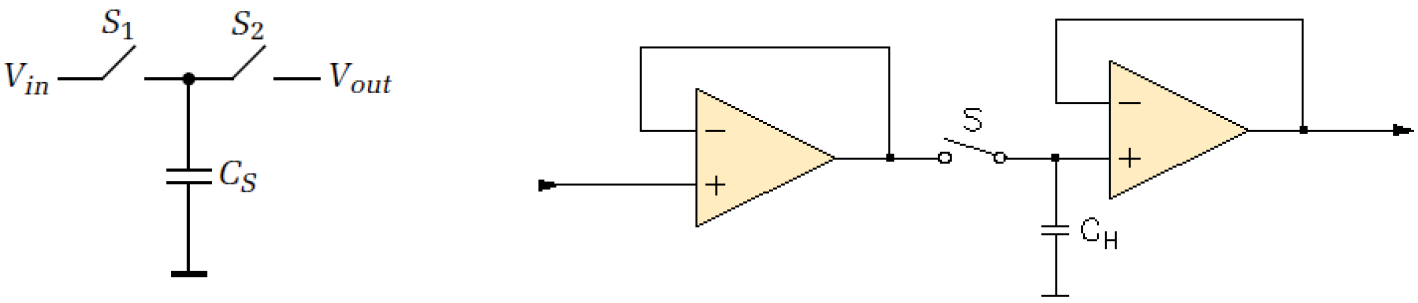
\includegraphics[width=0.8\columnwidth]{images/sample_hold.png}
\end{center}

\begin{tabular}{ll}
    links: & Belastung von Quelle und Senke \textrightarrow\ unbrauchbar! \\
    rechts & Ohne Belastung von Quelle und Senke (Buffer)  
\end{tabular}


\subsection{Parallelverfahren (Flash-Wandler)}

\subsubsection{3-Bit ADC nach Parallel-Verfahren (Flash-Wandler)}

\begin{minipage}[c]{0.38\columnwidth}
    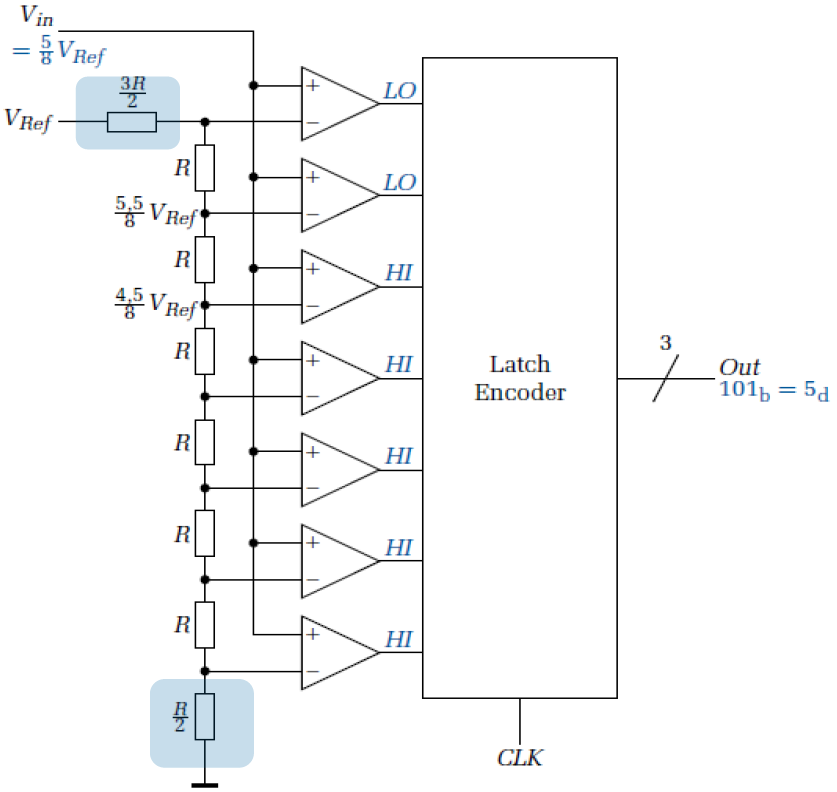
\includegraphics[width=\columnwidth]{images/ADC_parallelverfahren.png}
\end{minipage}
\hfill
\begin{minipage}[c]{0.6\columnwidth}
    \begin{itemize}
        \item[+] ADC ist \textbf{sehr schnell}
        \item[+] Nur 1 Takt
        \item[-] $2^n$ Widerstände
        \item[-] $2^n -1$ Komparatoren
    \end{itemize}
    
    \vspace{0.2cm}

    'Runden' ist möglich mit unterschiedlichen Widerständen ganz unten und ganz oben \cbl{(blau hinterlegt)} \\
    \cbl{ \textrightarrow\ 'Sprung' ist hier bei $\frac{q}{2}$ statt bei $q$}
\end{minipage}


\subsubsection{Pipeline- (Kaskaden-, Subranging-) ADC}

Kaskadierung von \textbf{Flash-ADCs}
\vspace{0.2cm} 

\begin{minipage}[c]{0.46\columnwidth}
    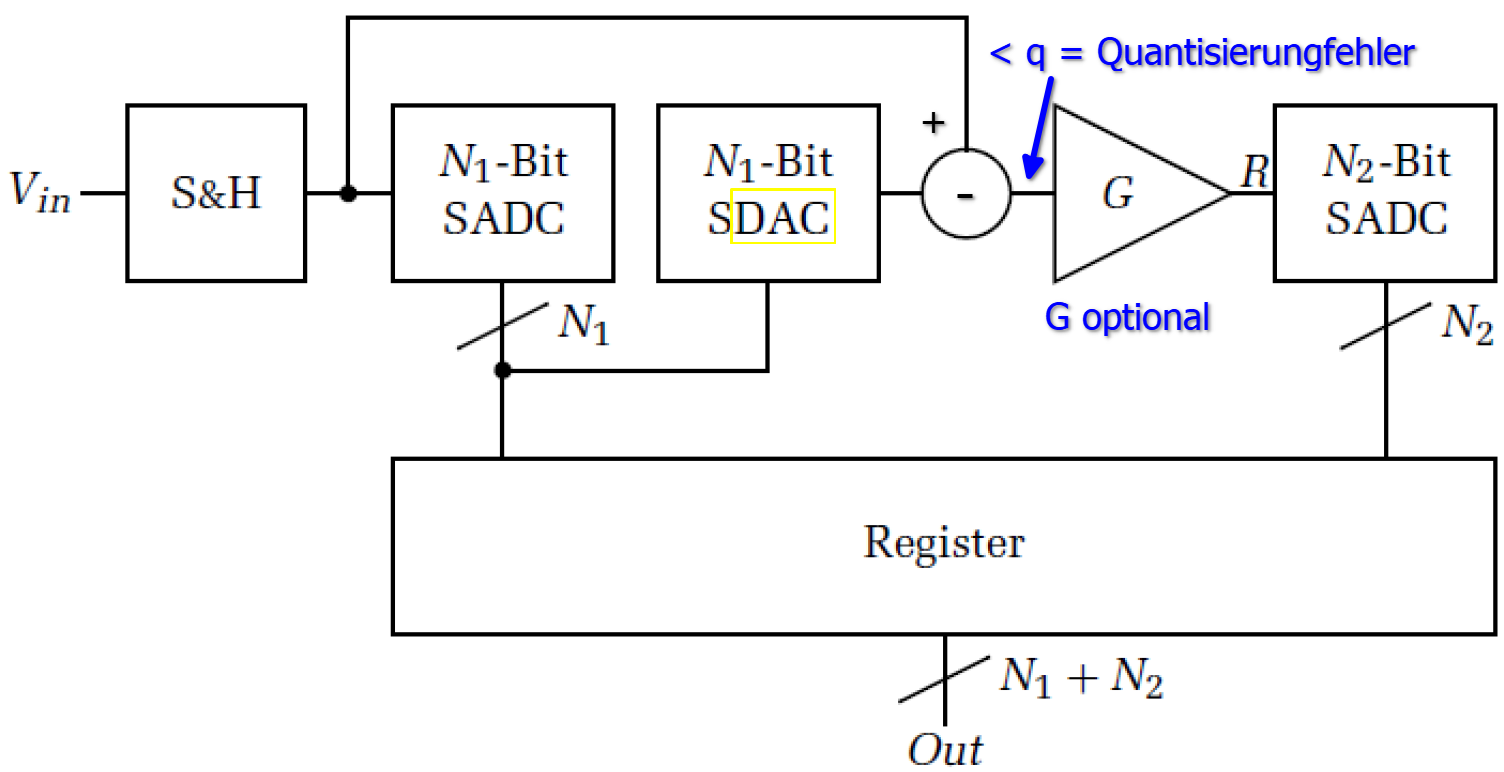
\includegraphics[width=\columnwidth]{images/pipeline_ADC.png}
\end{minipage}
\hfill
\begin{minipage}[c]{0.5\columnwidth}
    Zweistufig:

    \vspace{0.1cm}

    \begin{enumerate}
        \item ADC mit $N_1$ Bits
        \item ADC mit $N_2$ Bits
    \end{enumerate}

    \vspace{0.2cm}

    \begin{itemize}
        \item[+] Nur $2^{N_1} + 2^{N_2}$ Komparatoren
        \item[-] Braucht zusätzlichen DAC mit $N_1$ Bits
        \item[-] Braucht ev. Verstärker mit Gain $G$
    \end{itemize}
\end{minipage}

\vspace{0.2cm}

\myul{\textbf{Ablaufsteuerung Pipeline-ADC}}

\vspace{0.1cm}

\begin{minipage}[c]{0.33\columnwidth}
    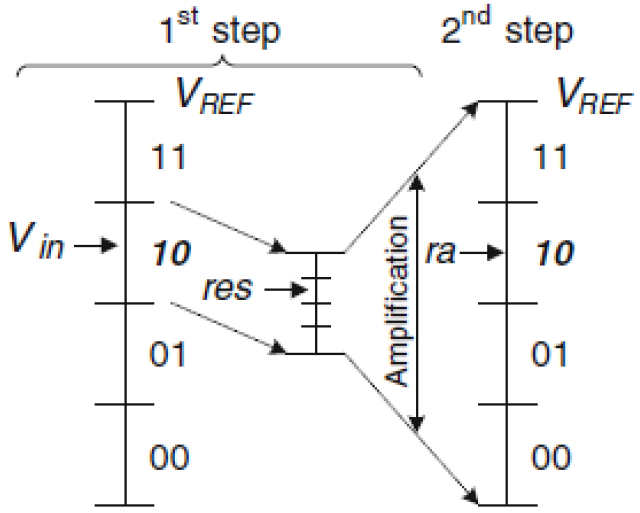
\includegraphics[width=\columnwidth]{images/ablauf_pipeline_ADC_2.png} 
\end{minipage}
\hfill
\begin{minipage}[c]{0.63\columnwidth}
    \begin{itemize}
        \item Spannungswert der digitalierten Spannung wird von $V_{\rm in}$ abgezogen
        \item Restspannung ($ < q$) wird mit $2^{N_1}$ multipliziert und digitalisiert mit $N_2$ Bits \\
            (bei gleicher Referenzspannung von 2. ADC)
    \end{itemize}
\end{minipage}


\subsubsection{Mehrstufiger Pipeline-Wandler}

\begin{center}
    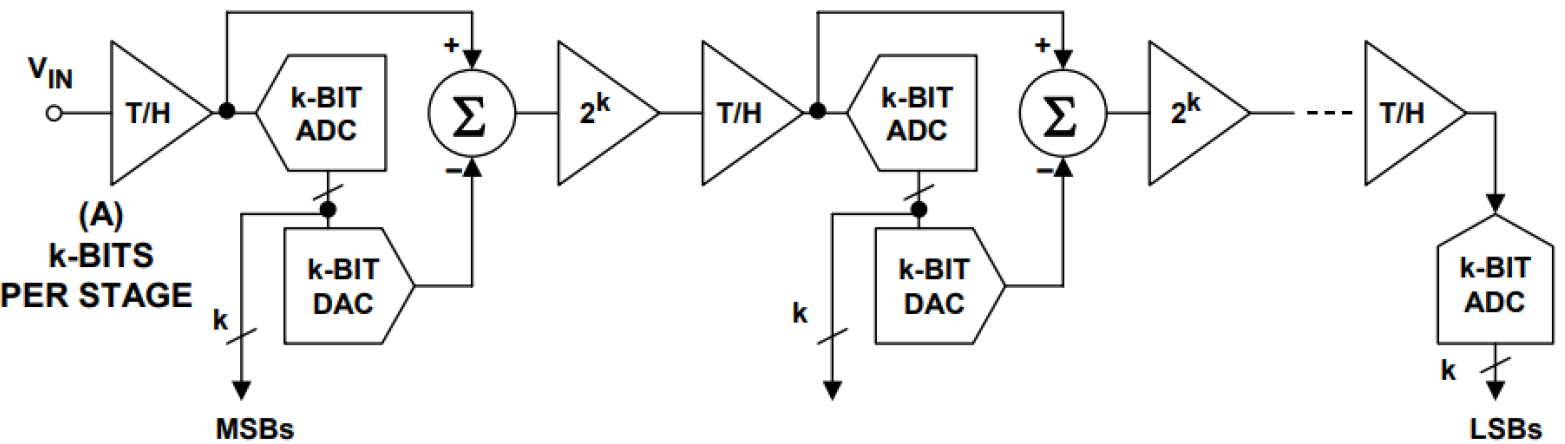
\includegraphics[width=0.8\columnwidth]{images/mehrstufiger_pipeline_wandler.png}
\end{center}


\begin{minipage}[c]{0.48\columnwidth}
    \begin{itemize}
        \item Flash-ADC mit $k \geq 1$ DAC mit $k$ Bits
        \item Multiplikation mit $2^k$ (gleiche Referenz für jede Stufe)
    \end{itemize}
\end{minipage}
\hfill
\begin{minipage}[c]{0.48\columnwidth}
    \begin{itemize}
        \item \textbf{Latenz bei $\bm{n}$ Stufen} \textrightarrow\ $n$ Zyklen
        \item Update-Frequenz $n$-mal grösser \\
            \textrightarrow\ In jedem Zyklus ein neuer Wert
    \end{itemize}
\end{minipage}

\vspace{0.2cm}

\textbf{Statt Multiplikation mit $\bm{2^k}$ kann auch die Referenzspannung der folgenden Stufe um $\bm{2^k}$ verkleinert werden!}


\subsubsection{Iterative ADC}

\begin{minipage}[c]{0.4\columnwidth}
    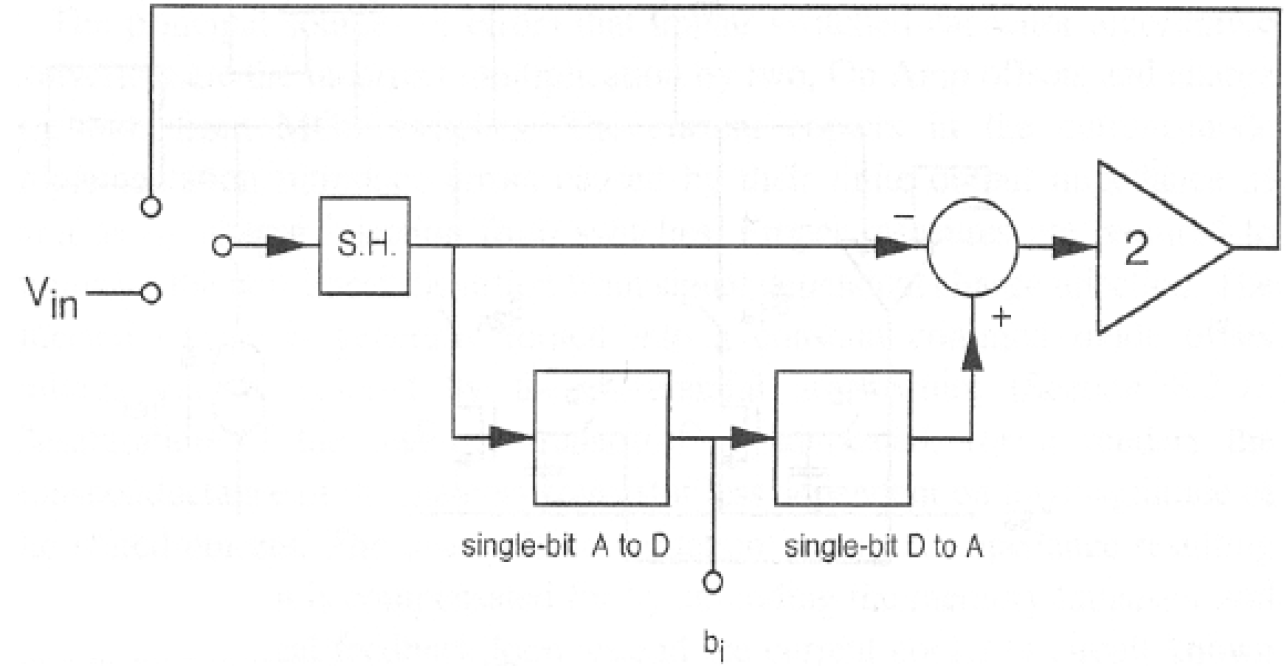
\includegraphics[width=\columnwidth]{images/iterativer_ADC}
\end{minipage}
\hfill
\begin{minipage}[c]{0.58\columnwidth}
    \raggedright
    Reststpannung (Quantisierungsfehler) verdoppeln, damit gleiche Referenzspannung verwendet werden kann 
\end{minipage}

\vspace{0.2cm}

\myul{\textbf{Ablauf einer Wandlung - Iterativer ADC} }

\vspace{0.1cm}

Mit \textbf{jedem Zyklus} (Loop) wird die \textbf{Auflösung um 1 Bit erhöht!}

\begin{minipage}[c]{0.27\columnwidth}
    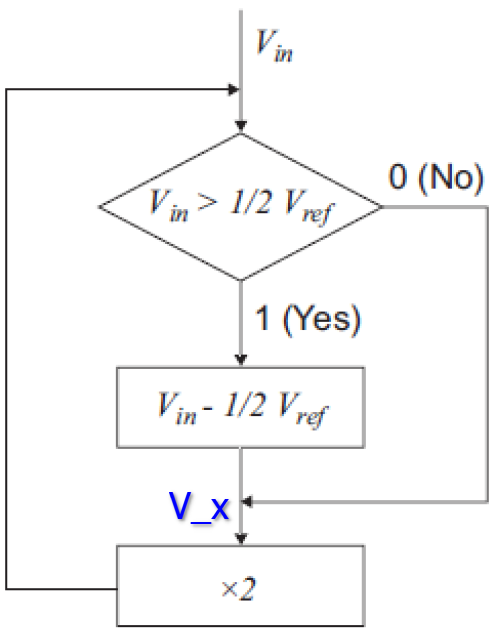
\includegraphics[width=\columnwidth]{images/iterativer_ADC_flussdiagramm.png} 
\end{minipage}
\hfill
\begin{minipage}[c]{0.72\columnwidth}
    \begin{outline}
        \1 Wenn $V_{\rm in} > \frac{V_{\rm ref}}{2}$
            \2 MSB$=1$, $\frac{V_{\rm ref}}{2}$ von $V_{\rm in}$ subtrahieren
            \2 $V_x = V_{\rm in} - \frac{V_{\rm ref}}{2}$
        \1 Wenn $V_{\rm in} < \frac{V_{\rm ref}}{2}$ 
            \2 MSB$=0$
            \2 $V_x = V_{\rm in}$
        \1 $V_x$ verdoppeln zur Bestimmung des nächsten Bits 
    \end{outline}
\end{minipage}


\subsection{Wägeverfahren}

\subsubsection{SAR: Sucessive Approximation Register}

\begin{minipage}[c]{0.35\columnwidth}
    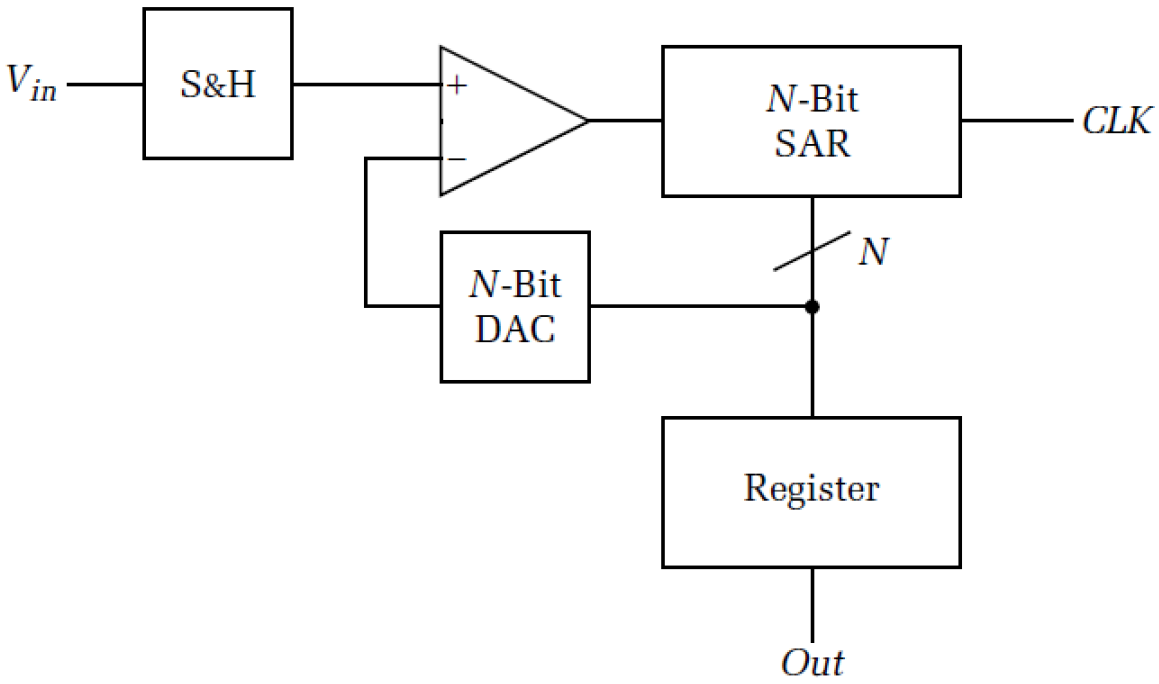
\includegraphics[width=\columnwidth]{images/SAR_ADC.png} 
\end{minipage}
\hfill
\begin{minipage}[c]{0.6\columnwidth}
    \begin{itemize}
        \item DAC-Ausgang nähert sich schrittweise dem Eingangssignal an
        \item Bei $n$ Bit Auflösung dauert eine Wandlung $n$ Zyklen
    \end{itemize}
\end{minipage}


\myul{\textbf{Beispiel Wandlung mit SAR-ADC}}

\vspace{0.1cm}

\begin{minipage}[c]{0.48\columnwidth}
    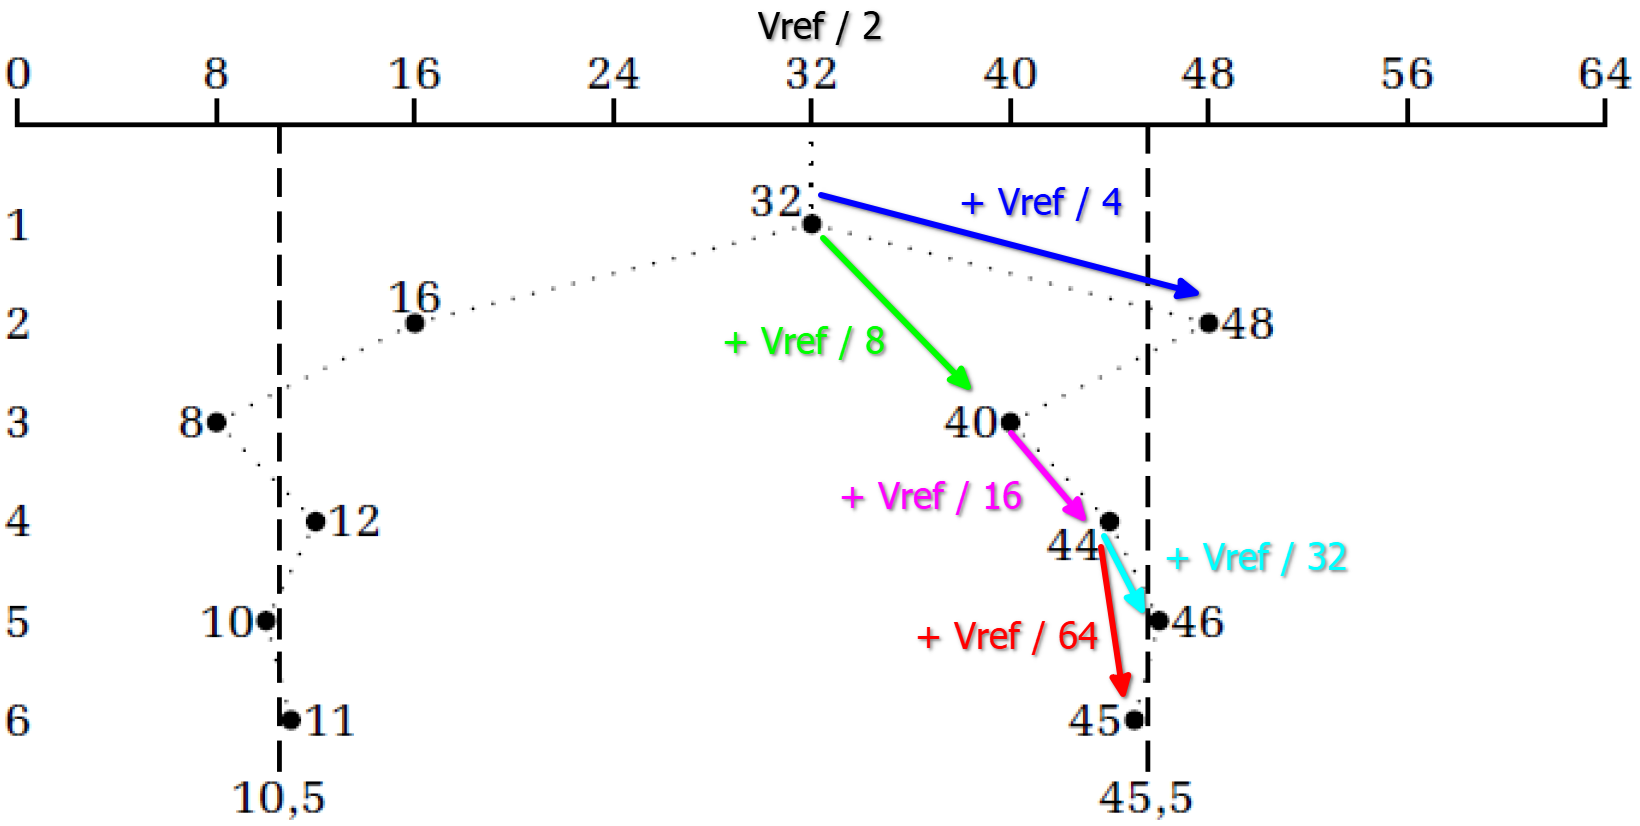
\includegraphics[width=\columnwidth]{images/SAR_ADC_beispiel.png} 
\end{minipage}
\hfill
\begin{minipage}[c]{0.48\columnwidth}
    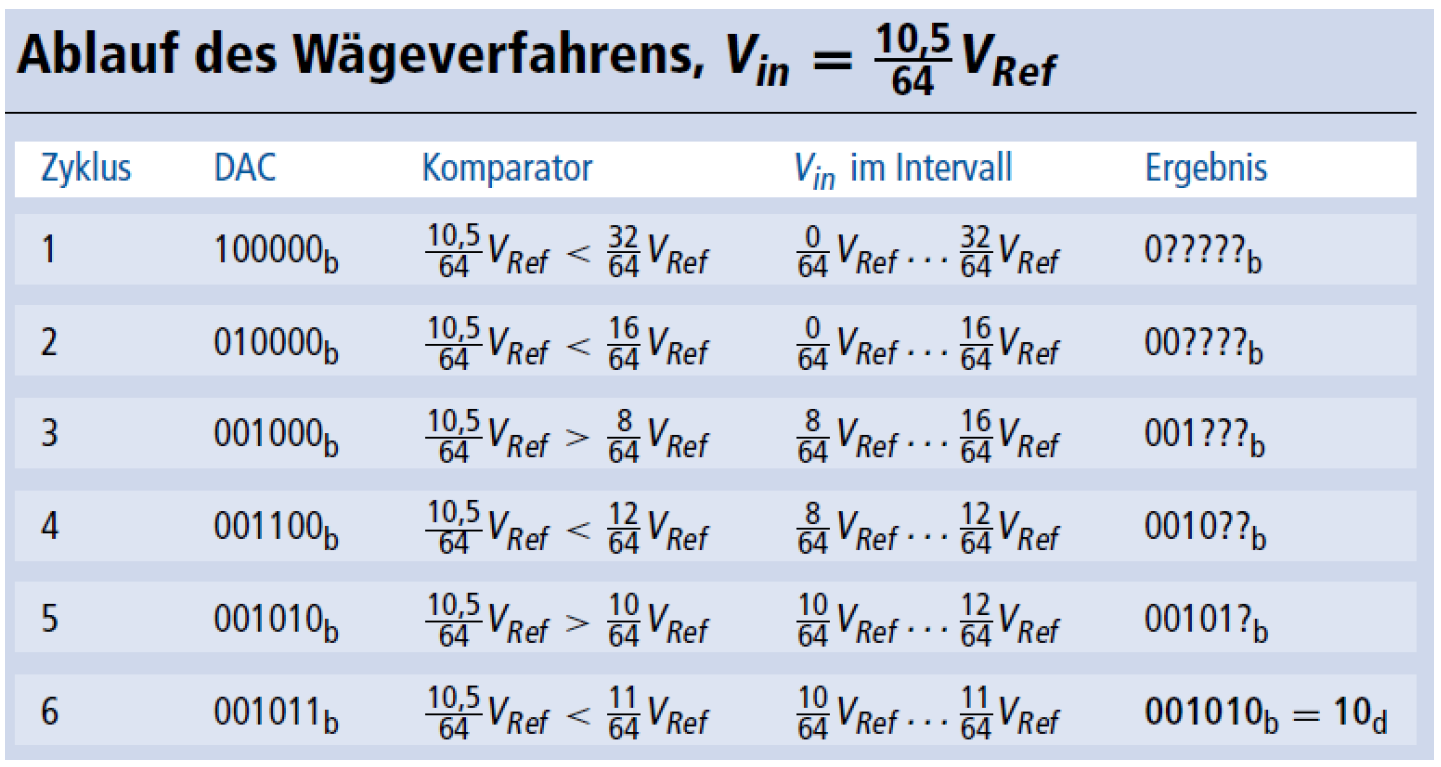
\includegraphics[width=\columnwidth]{images/SAR_ADC_beispiel_2.png} 
\end{minipage}


\subsubsection{SAR mit Switched Capacitor DAC (4 Bit)}

\begin{minipage}[c]{0.48\columnwidth}
    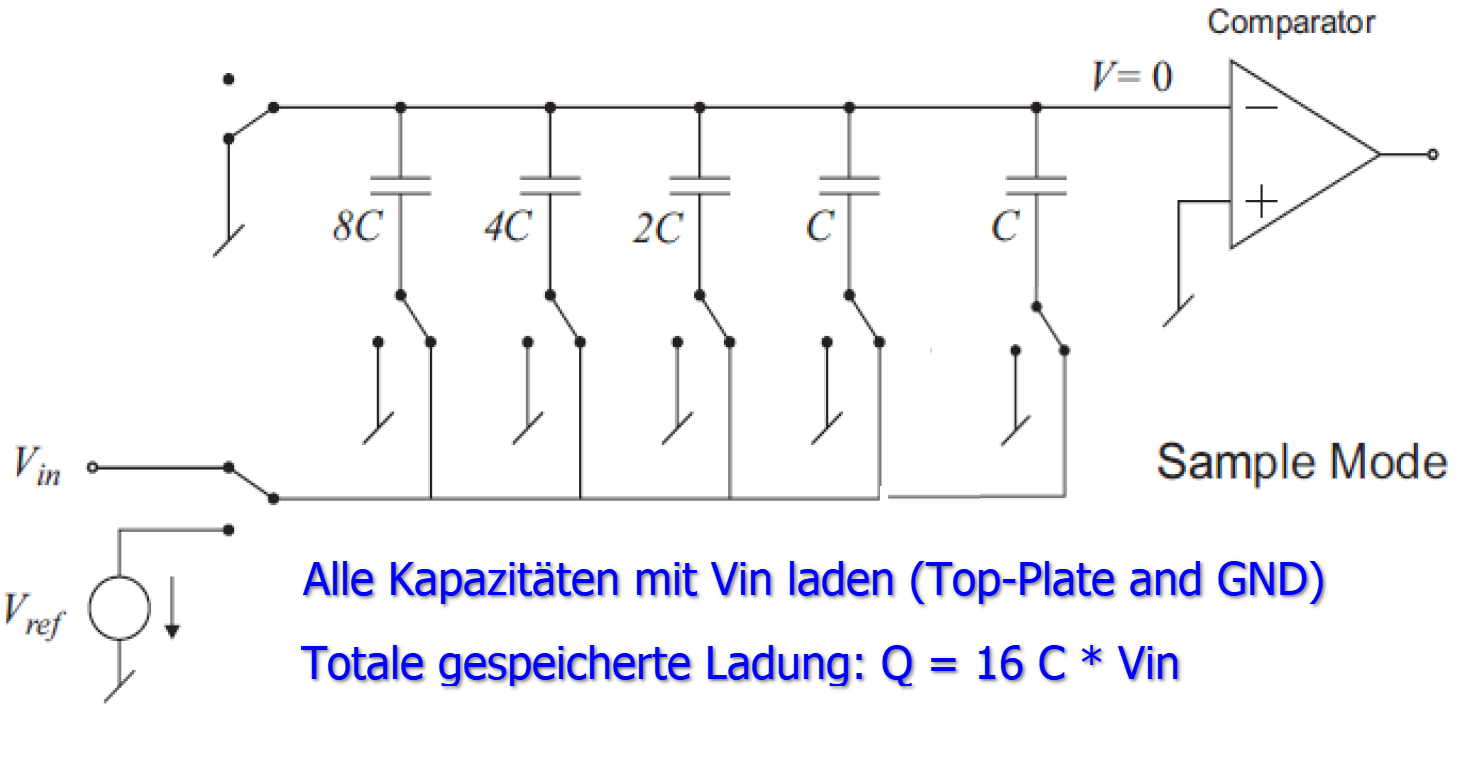
\includegraphics[width=\columnwidth]{images/SAR_switched_capacitor_sample_mode.png}
\end{minipage}
\hfill
\begin{minipage}[c]{0.48\columnwidth}
    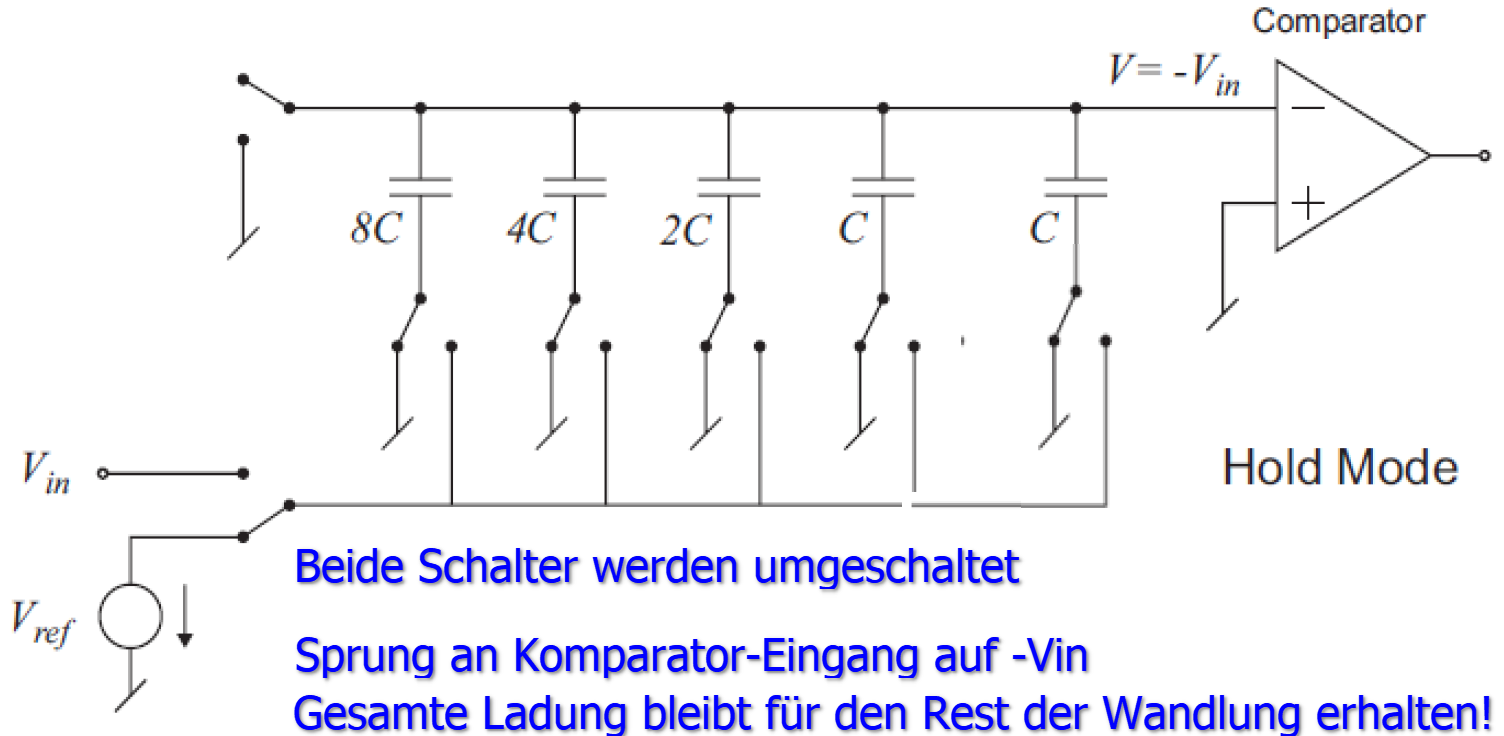
\includegraphics[width=\columnwidth]{images/SAR_switched_capacitor_hold_mode.png}
\end{minipage}

\begin{minipage}[c]{0.45\columnwidth}
    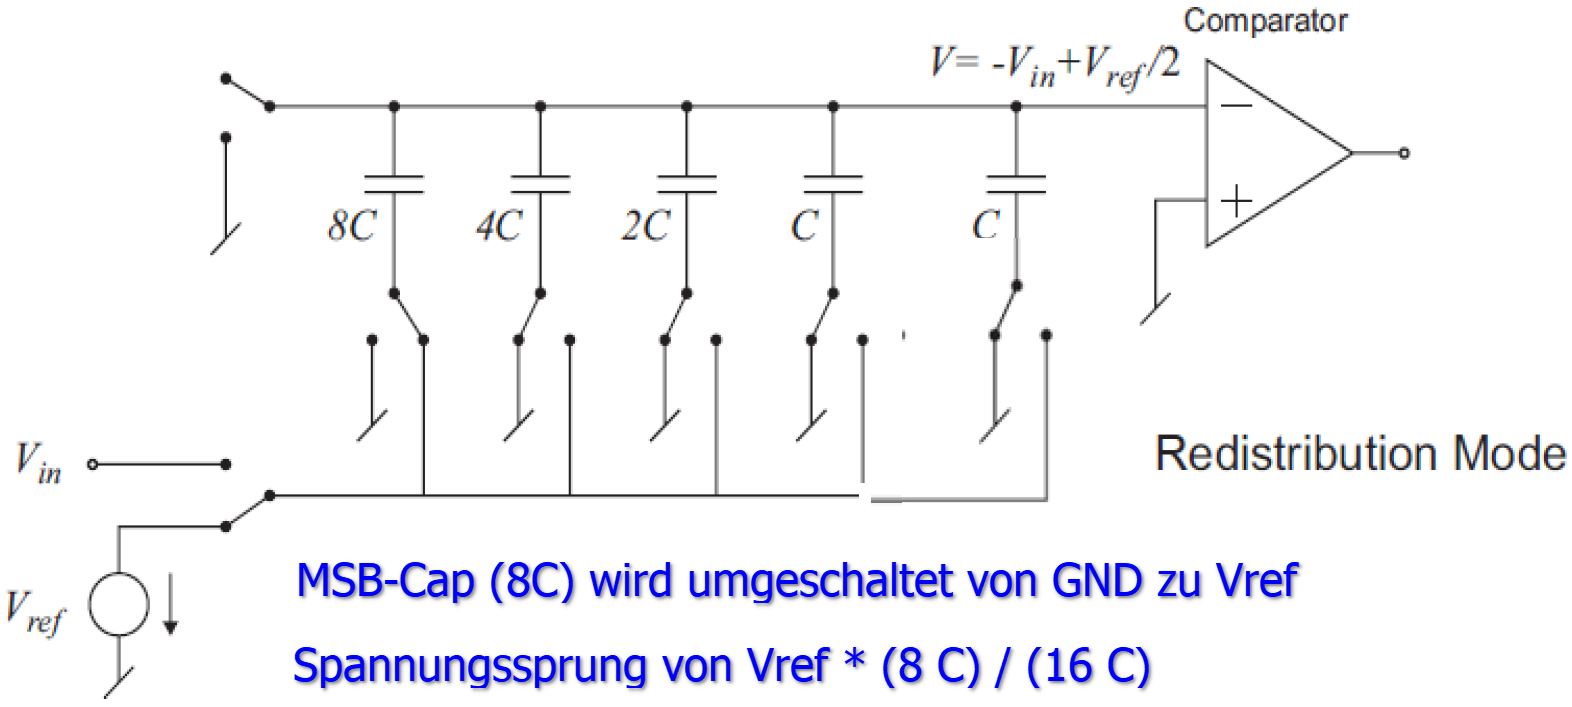
\includegraphics[width=\columnwidth]{images/SAR_switched_capacitor_redistribution_mode.png} 
\end{minipage}
\hfill
\begin{minipage}[c]{0.5\columnwidth}
    Komparator wird ausgewertet:

    \vspace{0.1cm}

    \begin{itemize}
        \item Falls $V < 0 \,V$: Bit = 1 \\
            \textrightarrow\ Schalter bleibt auf $V_{\rm ref}$
        \item Falls $V > 0 \,V$: Bit = 0 \\
            \textrightarrow\ Schalter  zurück auf GND
    \end{itemize}

    \vspace{0.1cm}

    Nächsten Schalter umlegen
\end{minipage}


\subsection{Zählverfahren}

\subsubsection{Grundprinzip: Zählverfahren}

\begin{minipage}[c]{0.4\columnwidth}
    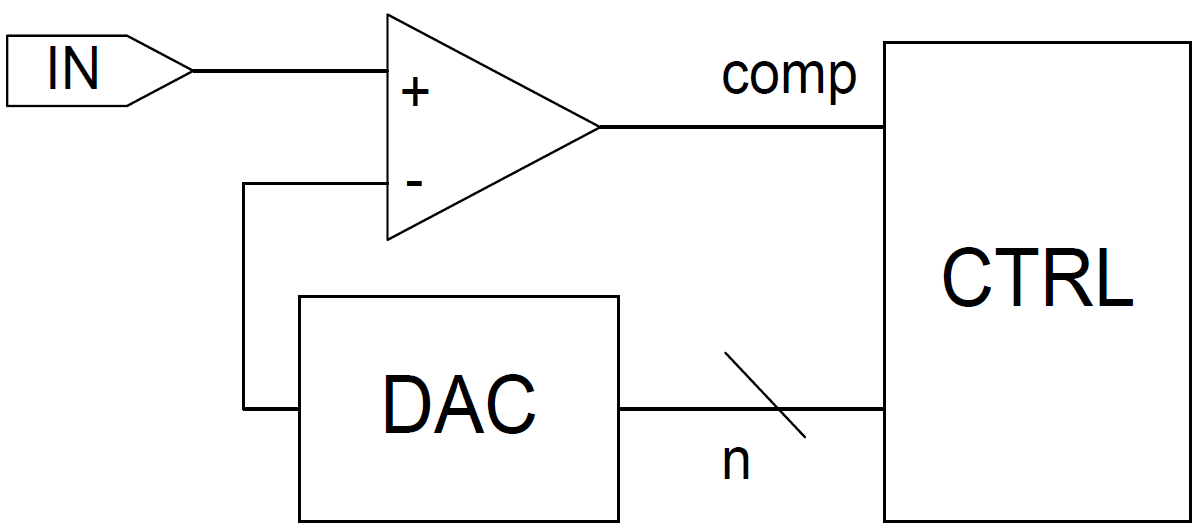
\includegraphics[width=\columnwidth]{images/ADC_zaehlverfahren_grundprinzip.png} 
\end{minipage}
\hfill
\begin{minipage}[c]{0.56\columnwidth}
    \raggedright
    \begin{itemize}
        \item CTRL zählt von $0$ bis $2^n -1$
        \item Zähler stoppt bei $\text{comp} = 0$
        \item \textbf{Zählstand = ADC-Wert} \\
            \textrightarrow\ 'aufgerundet', da DAC-Spannung grösser als $V_{\rm in}$
    \end{itemize}

\end{minipage}


\subsubsection{Single-Slope Wandler}

\begin{minipage}[c]{0.45\columnwidth}
    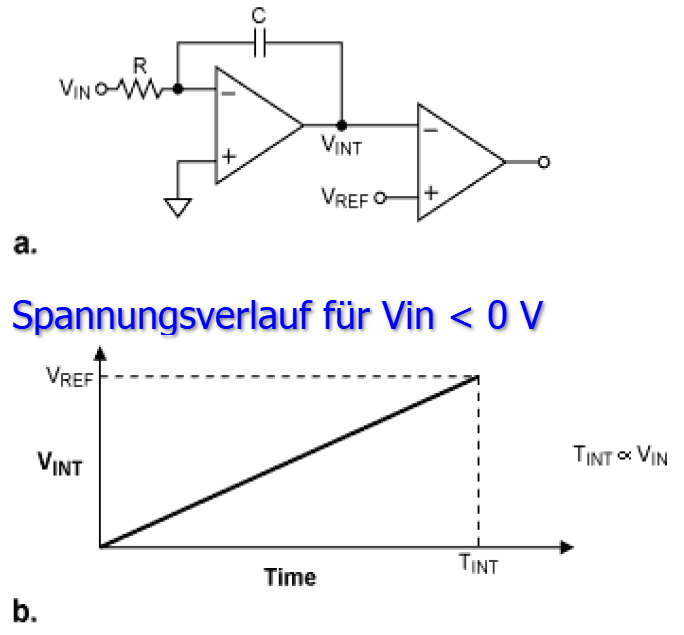
\includegraphics[width=\columnwidth]{images/single_slope_ADC.png} 
\end{minipage}
\hfill
\begin{minipage}[c]{0.52\columnwidth}
    Integration bis $ V_{\rm int}(t) = V_{\rm ref}$ 
    $$ \boxed{ V_{\rm int}(t) = - \frac{V_{\rm in} - A_{\rm GND} }{R \cdot C} \, t  + A_{\rm GND} } $$

    \vspace{0.1cm}

    Integrationszeit $T_{\rm int}$ 
    $$ \boxed{ T_{\rm int} = - \frac{V_{\rm ref} \cdot R \cdot C}{V_{\rm in} - A_{GND}} }$$ 
    $$ \boxed{ V_{\rm in} = - \frac{V_{\rm ref} \cdot R \cdot C}{ T_{\rm int}} } $$ 
\end{minipage}


\subsubsection{Dual-Slope Wandler}

\begin{minipage}[c]{0.42\columnwidth}
    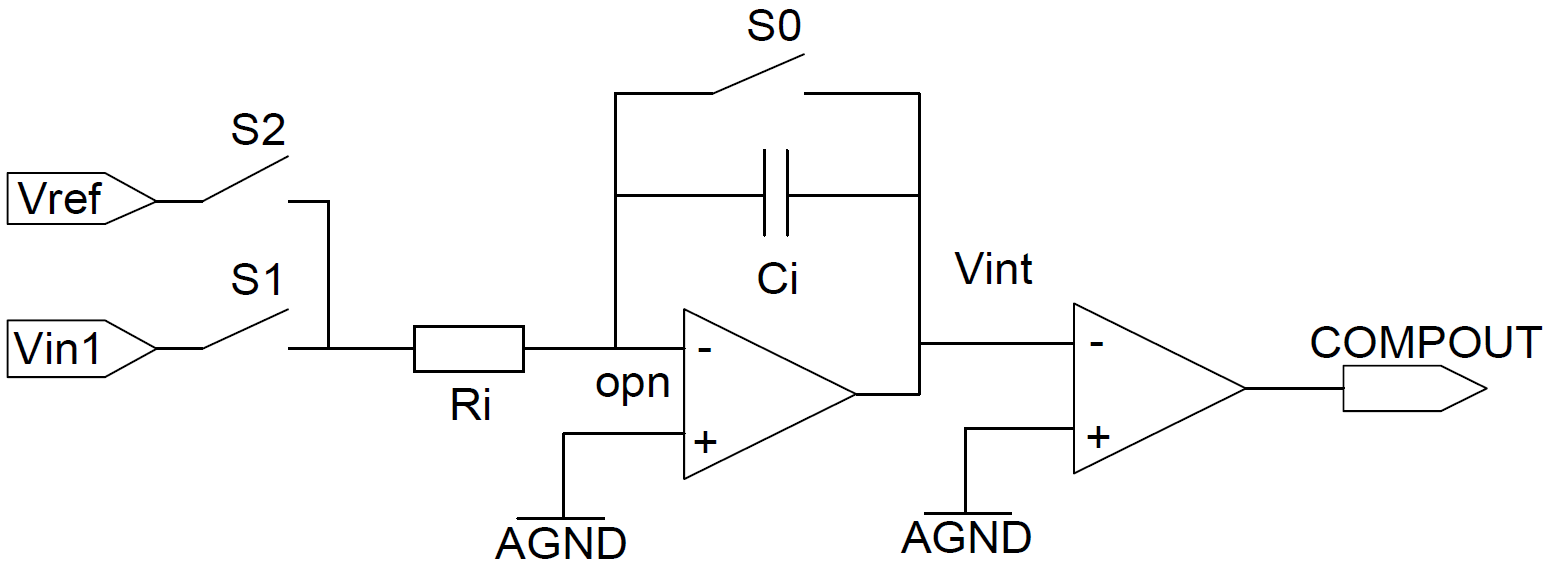
\includegraphics[width=\columnwidth]{images/dual_slope_ADC.png}
\end{minipage}
\hfill
\begin{minipage}[c]{0.27\columnwidth}
    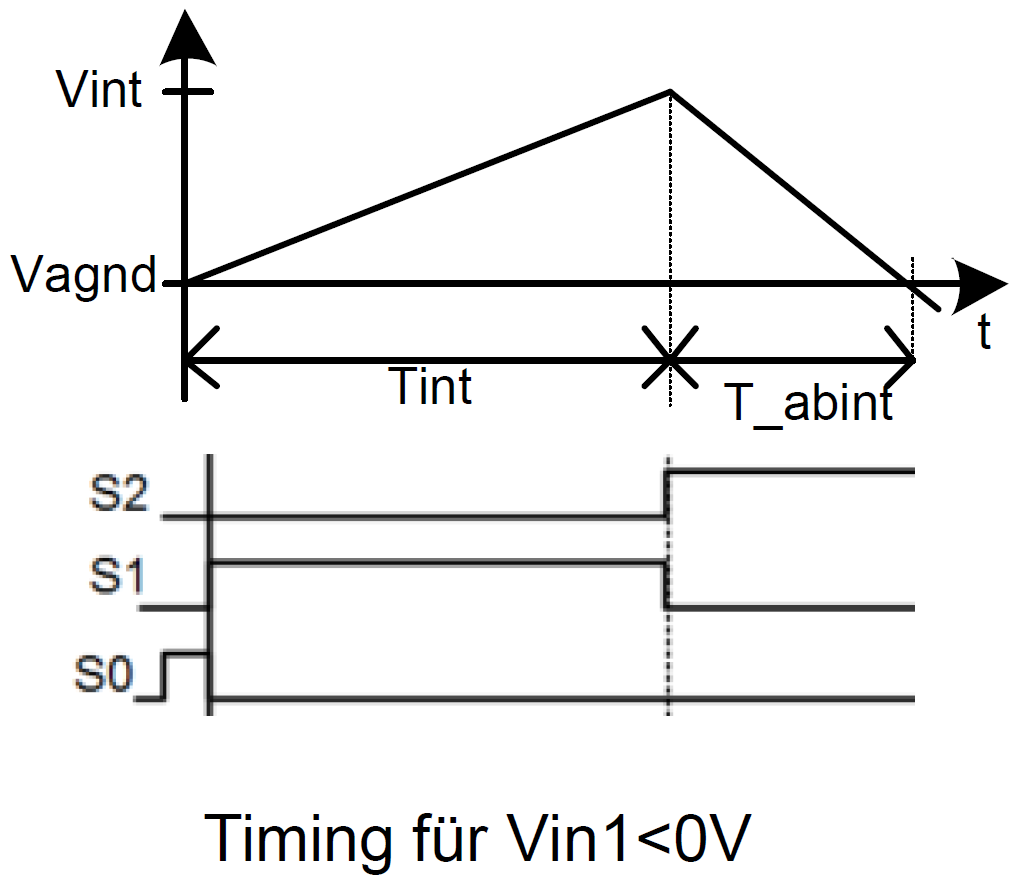
\includegraphics[width=0.83\columnwidth]{images/dual_slope_ADC_timing.png}
\end{minipage}
\hfill
\begin{minipage}[c]{0.29\columnwidth}
    $$ \boxed{ V_{\rm int} = \frac{\overline{V_{\rm in}} \cdot T_{\rm int}}{R_i \cdot C_i} } $$
    $$ \boxed{ V_{\rm abint} = \frac{V_{\rm ref} \cdot T_{\rm abint}}{R_i \cdot C_i}  } $$
\end{minipage}

$$ \boxed{ \text{DC: } V_{\rm int} = A_{\rm GND}- \frac{1}{R_i \cdot C_i} \, (V_{\rm in1}- A_{\rm GND}) \cdot T_{\rm int} }  $$
$$ \boxed{ \Delta V_{\rm abint} = A_{\rm GND} - V_{\rm int} = - \frac{1}{R_i \cdot C_i} \, (V_{\rm ref} - A_{\rm GND}) \cdot T_{\rm abint} } $$ 


\begin{minipage}[c]{0.33\columnwidth}
    $$ \boxed{ T_{\rm abint} = - \frac{V_{\rm in1} \cdot T_{\rm int}}{V_{\rm ref}} } $$ % mit V_AGND??
\end{minipage}
\hfill
\begin{minipage}[c]{0.3\columnwidth}
    $$ \boxed{ V_{\rm in1} = - V_{\rm ref} \frac{T_{\rm abint}}{T_{\rm int}} } $$ % mit V_AGND?
\end{minipage}
\hfill
\begin{minipage}[c]{0.3\columnwidth}
    $$ \boxed{ V_{\rm abint} = - V_{\rm int} } $$ %?
\end{minipage}

\begin{minipage}[c]{0.45\columnwidth}
    $$ \boxed{ -\frac{\overline{V_{\rm in}}}{V_{\rm ref}}= \frac{T_{\rm abint}}{T_{\rm int}} = \frac{n \cdot T_{clk}}{N \cdot T_{clk} } } $$
\end{minipage}
\hfill
\begin{minipage}[c]{0.53\columnwidth}
    $$ \boxed{ V_{\rm int} = \int\limits_0^{T_{\rm int}} - \frac{1}{R_i \cdot C_i} \, V_{\rm in1} + V_{\rm int,0} } $$
\end{minipage}

\vspace{0.2cm}

\myul{\textbf{Frequenzverhalten vom Dual-Slope-Wandler}}

\vspace{0.1cm}

Frequenzen $f = \frac{1}{T}$ , wobei $T$ der Intergrationszeit entspricht, werden perfekt unterdrückt \\
\textrightarrow\ Integrationszeit $T = 20 \, \milli \second$ unterdrückt Netzbrumm von $50 \, \hertz$


\subsubsection{Charge Balancing ADC (Sigma-Delta-Wandler)}

\begin{center}
    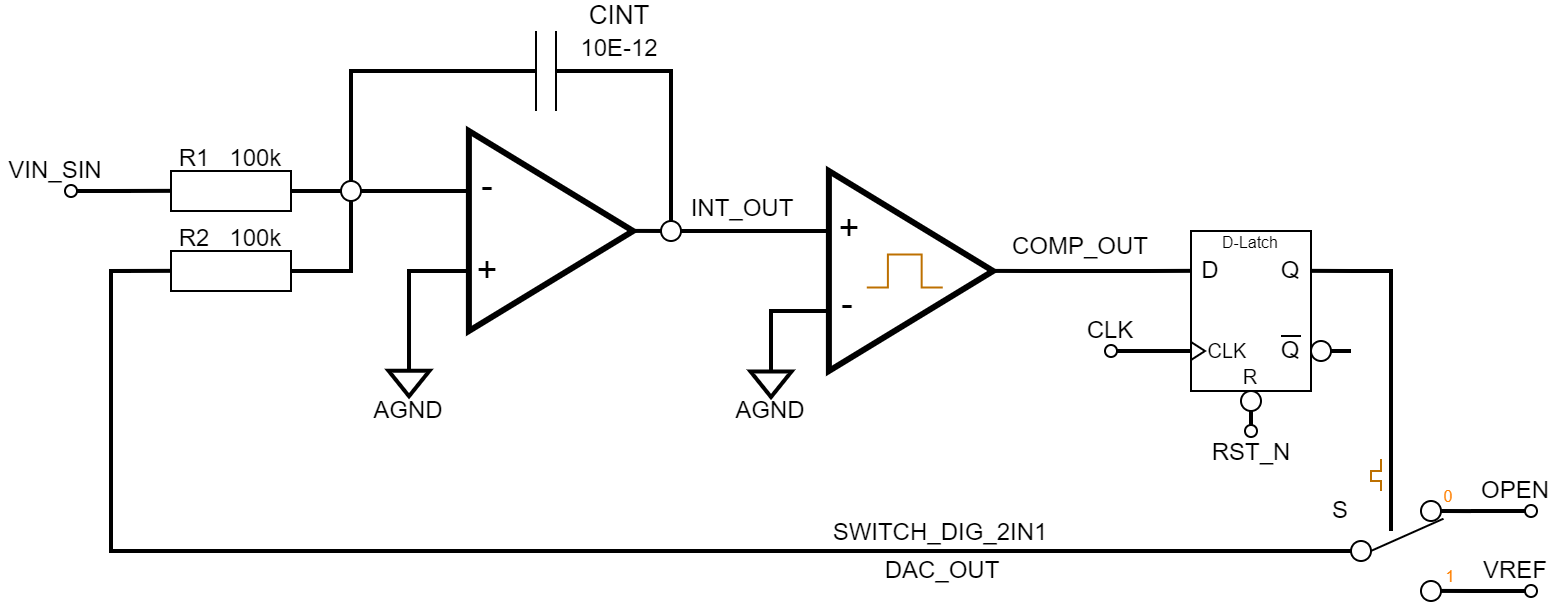
\includegraphics[width=0.8\columnwidth]{images/charge_balancing_ADC.png}
\end{center}


\begin{itemize}
    \item \textbf{Bei jedem Takt} während Aufintegration wird entschieden,
        ob fixe 'Ladungsportion' $Q$ abintegriert wird \textbf{(Schaltschwelle)} \\
        \textrightarrow\ Für CompOut $= 1$ wird für 1 CLK abintegriert
    \item Anzahl 'Ladungsportionen' zählen während $N$ Taktzyklen
    \item \textbf{Integration immer aktiv}
    \item Integrator-Ausgang im Schnitt = Schaltschwelle \textrightarrow\ $\diff Q = 0$
    \item Grosse $N$ \textrightarrow\ Lange Integrationszeit
\end{itemize}

$$ \boxed{ Q = \frac{T_{clk} \cdot V_{\rm ref}}{R_i} }  
    \qquad \boxed{ Q_{\rm int} = \frac{V_{\rm in} \cdot T_{\rm int}}{R_i \cdot C_i} } 
    \qquad \boxed{  \frac{\overline{V_{\rm in}}}{V_{\rm ref}} = \frac{T_{\rm abint}}{T_{\rm int}} = \frac{n}{N} } $$ 
$$ \boxed{ Q_{\rm abint} = \frac{V_{\rm ref} \cdot T_{\rm abint}}{R_i \cdot C_i} = - Q_{\rm int} } $$ 


\subsubsection{Fazit Integrierende Wandler}

\begin{itemize}
    \item In einem Messzyklus wird gleich viel Ladung vom Eingang wie von der Referenzspannung aufintegriert
    \item Sigma-Delta-Wandler können in kürzerer Zeit hohe Auflösungen erreichen als Dual-Slope Wandler 
\end{itemize}


\subsection{Abtastung und Quantisierung}

\begin{tabular}{ll}
\textbf{Aliasing}       & Abgetastetes Signal kann sauber rekonstruiert werden, \\
                        & aber auch schnellere Signale können gleiche Abtastwerte haben \\
\textbf{Abtasttheorem}  & $\bm{f_{\rm abtast} > 2 \cdot f_{\rm signal,max}}$ \\
\textbf{Sample-Hold}    & S-H-Glieder wirken wie Tiefpassfilter, indem das Spektrum mit \\
                        & einer sinc-Funktion $(\sin(x)/x)$ gewichtet wird  \\
                        & \textrightarrow\ ALLE Frequenzen $> 0 \, \hertz$ werden durch S-H gedämpft! \\
                        & (gutes S-H = wenig Dämpfung)
\end{tabular}


\subsection{Lineares Modell der Quantisierung / SNR}

\subsubsection{Voraussetungen für lineare Modellierung der Quantisierung}

\begin{itemize}
    \item Anzahl der Bits $N$ ist gross
    \item ADC wird nicht übersteuert $(V_{\rm refn} < V_{\rm in} < V_{\rm refp})$
    \item Alle Spannungen kommen in Eingangssignal gleich oft vor
    \item Analoges Eingangssignal variiert sehr schnell
\end{itemize}


\subsubsection{Signal-Rausch-Abstand (SNR)}

\begin{itemize}
    \item \textbf{SNR:} Verhältnis Signalleistung zu Quantisierungsrauschen \textbf{in dB}
    \item ENOB: Effevtive Number of Bits
\end{itemize}

\vspace{0.2cm}

\renewcommand{\arraystretch}{1.5}
\begin{tabular}{ll}
    Leistung Quantisierungsrauschen & $P_Q = \frac{q^2}{12}$                                            \\
    Leistung Eingangssignal         & $P_S = 2^{2 \cdot n - 3} \cdot q^2$                               \\
    SNR                             & $1.76 + n \cdot 6.02$ mit $n =$ \# Bits                           \\
    ENOB                            & $\mathrm{ENOB} = \frac{\mathrm{SNR_{\deci \bel}} - 1.76}{6.02}$ 
\end{tabular}
\renewcommand{\arraystretch}{1}

\vspace{0.2cm}

\textbf{ \textrightarrow\ Pro Bit erhöht sich SNR um 6.02 dB}
 
 
\subsection{Kennwerte von ADCs}

\begin{center}
    \begin{tabular}{lccc}
        \toprule
                                    & \textbf{Pipelined}    & \textbf{Wägeverfahren}    & \textbf{Sigma-Delta}      \\
        \midrule
        \textbf{Auflösung}          & niedrig               & mittel                    & hoch                      \\  
                                    & 8 - 14 Bit            & 8 - 20 Bit                & 16 - 24 Bit               \\
        \midrule
        \textbf{Umsetzungsrate}     & sehr hoch             & mittel-hoch               & niedrig-mittel            \\
                                    & bis zu 4 GSa          & bis zu 10 MHz             & 1 Hz - 100 kHz            \\
        \midrule
        \textbf{Leistungsaufnahme}  & sehr hoch             & mittel                    & niedrig                   \\
                                    & bis zu 3 W            & 1 - 200 mW                & 0.2 - 10 mW               \\
        \bottomrule
    \end{tabular}
\end{center}

